\begin{problem}{Autograd from Scratch \hfill {[20 pts]}}{prob:autograd}
\label{prob:autograd}

In this problem, you will implement your very own \textit{scalar autograd}
(differentiation) library. If you're scared, don't be! You'll be writing just
100-150 lines of Python code in 2 files. This problem aims to introduce you to
automatic differentiation and backpropagation by demonstrating how they work at
the scalar (single number) level. More advanced libraries like PyTorch, JAX, and
TensorFlow/Keras extend these concepts to the tensor/matrix/vector levels for
automatic differentiation. This assignment is inspired and adapted from Andrej
Karpathy's \verb|micrograd| \cite{Andrej2024karpathy}.

\vspace{10px}
\textbf{Setup}

Download the assignment \verb|.zip| from Gradescope and extract it somewhere on
your computer. Follow the project setup in \verb|SETUP.md|. It'll guide you on
how to install \verb|graphviz| and \verb|uv|, which we'll be using to manage
your python environment. We've also made a setup video guide
\href{https://youtu.be/9R_9iv-Y4Ts}{here}.

\vspace{10px}
\textbf{Automatic Differentiation}

Say we have an expression $y = ax + b$. We know that $\frac{\partial y}{\partial
x} = a$ or $\frac{\partial{y}}{\partial a} = x$ or $\frac{\partial y}{\partial
b} = 1$, but how do we calculate these partial derivatives automatically? What
about far more complex expressions with nested structures?\\

The idea is to wrap constants and variables (to us they are all unit values)
like $a, b, x$ in a \verb|Value| object/class (which you will implement), to
exploit the modularity of both the "forward" and "backward" computation logic.
So $3.14 \rightarrow \verb|Value(3.14)|$. Then, we can construct complex
expressions with these unit \verb|Value|'s as building blocks. Under the hood,
we will automatically construct a computation graph (DAG) as visualized in
\cref{fig:handbackprop}. \verb|Value| objects have methods that allow them to
interact with other \verb|Value|'s. For instance, you will implement functions
for adding, subtracting, multiplying, and dividing any two \verb|Value| objects
as well as special transformations called \textit{non-linearities} (ReLU,
Sigmoid, tanh). For example, $\verb|Value(3.14).sigmoid()| = \sigma(3.14) =
\frac{1}{1 + e^{-3.14}}$. Finally, you will implement the backbone of the
autograd engine, the \verb|backward()| method, which relies on the computation
graph we constructed when piecing together values.\\

\vspace{10px}
\textbf{Gradient Back-propagation}

To find the gradient of the loss function $L$ with respect to a parameter $w$,
we use the chain rule. $w_{next}$ is the node right after the current parameter
$w$, so in \cref{fig:handbackprop} if $w=w_1$ then $w_{next}=s$.

\[
\frac{\partial L}{\partial w} = 
\underbrace{\frac{\partial L}{\partial w_{next}}}_{\text{Gradient of next value.}} \cdot 
\underbrace{\frac{\partial w_{next}}{\partial w}}_{\text{Local gradient}}
\]


Start by reading \verb|grad/autograd.py|. Understand the \verb|__init__|,
\verb|__repr__|, \verb|parse|, and \verb|__add__| functions in the \verb|Value|
class.\\

Implement the following functions to enable \texttt{Value} operations. We've
done \verb|__add__| and \verb|__radd__| for you already, so read through those
first. If you don't follow a similar order/structure, we cannot guarantee that
your tests will pass. To understand what \verb|__radd__| does, read the first
response to
\href{https://www.reddit.com/r/learnpython/comments/3cvgpi/can_someone_explain_radd_to_me_in_simple_terms_i/}{this
thread}. Run tests with \verb|uv run tests.py| or \verb|python tests.py| from
the root directory after you implement each function! These functions are
methods of the \verb|Value| class, so \verb|self| refers to the current object,
and \verb|other| refers to the other object. For example, Python maps
\verb|val_a + val_b| to the \verb|__add__| function with \verb|self=val_a| and
\verb|other=val_b|.\\

\textbf{CAREFUL:} When updating \verb|self.grad| in these parts, use
\verb|self.grad +=| instead of \verb|self.grad =| because the same \verb|Value|
can be used twice in an expression, so we should be accumulating gradients, not
overwriting what's already in a \verb|Value|'s \verb|self.grad| field.

\begin{adjustwidth}{2em}{2em}
    \textbf{(a)} \verb|__mul__| (self * other) \hfill (2 pts)\\
    \textbf{(b)} \verb|__sub__| (self - other) \hfill (2 pts)\\
    \begin{adjustwidth}{2em}{2em}
    hint: addition and negation\\
    \verb|__neg__| is already implemented for you\\
    \end{adjustwidth}
    \textbf{(c)} \verb|__pow__| (self ** other) \hfill (2 pts)\\
    \textbf{(d)} \verb|__truediv__| (self / other) hint: multiplication and
    power \hfill (2 pts)\\
\end{adjustwidth}

Now you'll implement some non-linear transformations, often called
\textit{nonlinearities}. Specifically, you'll implement the ReLU, sigmoid, and
tanh transformations. We use these non-linear transformations later when
building neural networks. Where possible, try to reuse code by calling the
earlier functions. Some functions and derivatives can be represented in terms of
themselves, or other previously handled cases. You may use the \verb|math|
library to compute values of tanh(x) or exp(x).

\vspace{10px}
\begin{adjustwidth}{2em}{2em}
    \textbf{(e)} \verb|f_relu| \hfill (2 pts)\\
    \textbf{(f)} \verb|f_sigmoid| \hfill (2 pts) \\
    \textbf{(g)} \verb|f_tanh| \hfill (2 pts)\\
\end{adjustwidth}
\vspace{10px}


To the final part of this problem! Implement the following\ldots

\vspace{10px}
\begin{adjustwidth}{2em}{2em}
\textbf{(h)} \verb|backward| \hfill (3 pts)\\
\textbf{(i)} {Compare with hand-backpropagation} \hfill (3 pts)\\

\begin{adjustwidth}{2em}{2em}
You will complete a few lines in \verb|examples/ex_2i_backprop.py|. In
problem 1, we did backpropagation by hand, for the expression $L = (w_1 +
w_2) \cdot w_3$. Recreate this same expression from \cref{fig:handbackprop}
and complete all TODOs. Run the script to generate
\verb|figs/ex_backprop_before.png| and \verb|figs/ex_backprop_after.png|.
Include both in your submission and comment on whether the calculated
gradients, updated parameters $w_1,w_2,w_3$, and new result value $L$ match
with your previous results in Problem 1.\\
\end{adjustwidth}

\vspace{10px}
You've successfully implemented an autograd engine that is capable of minimizing
any expression that can be composed by your \verb|Value| class (which supports
basic operations, in addition to three non-linearities). Notice that any loss
function $L$ that can be defined in terms of \verb|Value|'s  can be minimized
with our autograd library.\\
    
\end{adjustwidth}
\vspace{10px}
\end{problem}


\begin{solution*}{}{}
\begin{center}
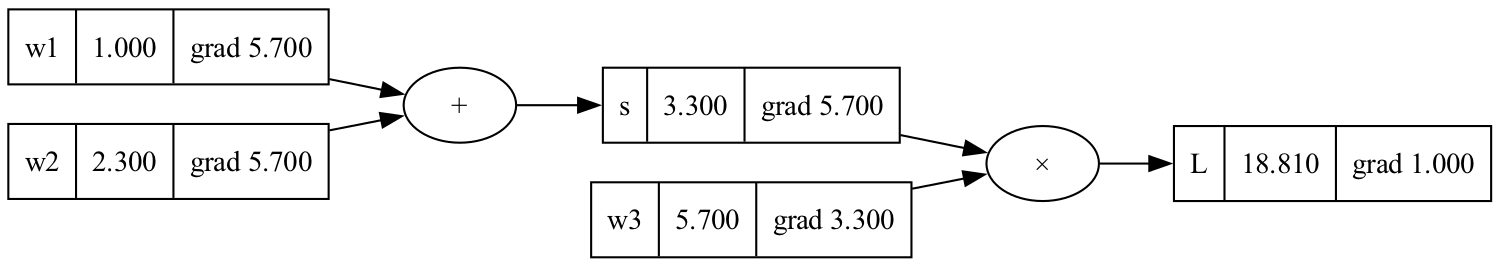
\includegraphics[width=\textwidth]{../figs/ex_backprop_before.png}
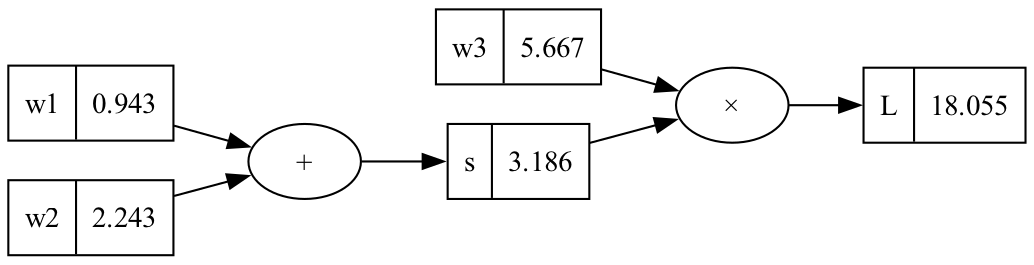
\includegraphics[width=\textwidth]{../figs/ex_backprop_after.png}
\end{center}
\end{solution*}
